\documentclass[11pt, letterpaper]{article}

% ── Packages ──
\usepackage[utf8]{inputenc}
\usepackage[T1]{fontenc}
\usepackage{amsmath, amssymb, amsthm, mathtools}
\usepackage{microtype}
\usepackage{newtxtext,newtxmath}
\usepackage{geometry}
\usepackage{graphicx}
\usepackage{hyperref}
\usepackage{enumitem}
\usepackage{booktabs}
\usepackage{array}
\usepackage{caption}
\usepackage{algorithm}
\usepackage{algpseudocode}
\usepackage[svgnames]{xcolor}
\usepackage{titling}
\usepackage{titlesec}

\geometry{margin=1.05in}
\graphicspath{{figures/}}
\hypersetup{
  colorlinks=true,
  linkcolor=MidnightBlue,
  citecolor=MidnightBlue,
  urlcolor=MidnightBlue,
  pdftitle={A Lasserre SDP Lower Bound for the Autoconvolution Constant},
  pdfauthor={Andrei Piterbarg and Jai Bajaj},
  pdfsubject={A Lasserre SDP lower bound for the autoconvolution constant}
}
\captionsetup{font=small, labelfont=bf}
\setlist{topsep=4pt, itemsep=2pt, parsep=0pt}
\setlength{\parindent}{1.1em}
\setlength{\parskip}{0pt}
\allowdisplaybreaks
\setlength{\droptitle}{-2.8em}
\pretitle{\begin{center}\LARGE}
\posttitle{\par\end{center}\vspace{-0.65em}}
\preauthor{\begin{center}\normalsize}
\postauthor{\par\end{center}\vspace{-0.45em}}
\predate{\begin{center}\small}
\postdate{\par\end{center}\vspace{0.6em}}

\titleformat{\section}
  {\normalfont\Large\bfseries}
  {\thesection.}{0.55em}{}
\titleformat{\subsection}
  {\normalfont\large\bfseries}
  {\thesubsection.}{0.5em}{}
\titlespacing*{\section}{0pt}{2.2ex plus 0.8ex minus 0.3ex}{1.0ex}
\titlespacing*{\subsection}{0pt}{1.6ex plus 0.5ex minus 0.2ex}{0.7ex}

% ── Theorem environments ──
\newtheoremstyle{paperplain}
  {8pt}{8pt}{\itshape}{}{\bfseries}{.}{0.5em}{}
\newtheoremstyle{paperdef}
  {8pt}{8pt}{\normalfont}{}{\bfseries}{.}{0.5em}{}
\theoremstyle{paperplain}
\newtheorem{theorem}{Theorem}[section]
\newtheorem{lemma}[theorem]{Lemma}
\newtheorem{proposition}[theorem]{Proposition}
\newtheorem{corollary}[theorem]{Corollary}
\newtheorem{claim}[theorem]{Claim}
\theoremstyle{paperdef}
\newtheorem{definition}[theorem]{Definition}
\newtheorem{remark}[theorem]{Remark}
\newtheorem{example}[theorem]{Example}

% ── Macros ──
\newcommand{\R}{\mathbb{R}}
\newcommand{\N}{\mathbb{N}}
\newcommand{\Z}{\mathbb{Z}}
\newcommand{\E}{\mathbb{E}}
\newcommand{\Linf}{L^\infty}
\newcommand{\supp}{\operatorname{supp}}
\newcommand{\tv}{\operatorname{tv}}
\newcommand{\val}{\operatorname{val}}
\DeclareMathOperator{\tr}{tr}
\newcommand{\PSD}{\succeq 0}

% ══════════════════════════════════════════════════════════════════════
\title{\texorpdfstring{%
  \bfseries A Lasserre SDP Lower Bound for the Autoconvolution Constant $C_{1a}$
}{A Lasserre SDP Lower Bound for the Autoconvolution Constant C1a}}
\author{Andrei Piterbarg \\ Jai Bajaj}
\date{}

\begin{document}
\maketitle

\begin{abstract}
We prove that the autoconvolution constant
\[
  C_{1a}
  \;=\;
  \inf_f \frac{\|f*f\|_{L^\infty}}{\left(\int f\right)^2},
\]
taken over nonnegative functions supported on $(-\tfrac14,\tfrac14)$,
satisfies $C_{1a}\ge 1.3$.  The proof reduces the infinite-dimensional
optimization to the polynomial program
\[
  \val(d)
  \;=\;
  \min_{\mu \in \Delta_d}\;\max_W \mu^\top M_W\,\mu,
\]
where $\Delta_d$ is the standard simplex and $\{M_W\}$ is a finite
family of nonnegative matrices encoding windowed autoconvolution test
values.  We show $\val(d) \le C_{1a}$ for every $d$, then certify
$\val(d)\ge 1.3$ at $d=16$ via the order-$3$ Lasserre
hierarchy~\cite{Lasserre2001}.  At higher resolutions we replace
the full moment cone by its correlative-sparsity
restriction~\cite{Waki2006}, which preserves soundness while
accommodating numerical corroboration at $d\in\{32,64,128\}$.  The
external dependency of the proof is a single finite SDP at
$(d,k)=(16,3)$ whose dual solution we record as the certificate.
\end{abstract}
\noindent\textit{2020 Mathematics Subject Classification.}
11B83, 42A85, 90C22, 90C23.

\smallskip

\noindent\textit{Keywords.}
Autoconvolution, Sidon sets, Lasserre hierarchy, sum-of-squares,
semidefinite programming, correlative sparsity, computer-assisted
proof.

\medskip

% ======================================================================
\section{Introduction}\label{sec:intro}
% ======================================================================

\subsection{The Constant \texorpdfstring{$C_{1a}$}{C1a}}

All source code and the SDP certificate are available at the
accompanying repository.  Let
\[
  \mathcal{F}
  \;=\;
  \left\{
    f \in L^1(\R) :
    f \ge 0,\
    \supp(f) \subseteq \left(-\tfrac14,\tfrac14\right),\
    \int_{\R} f > 0
  \right\}.
\]
For $f\in\mathcal{F}$ the \emph{autoconvolution} $(f*f)(t) =
\int f(x)f(t-x)\,dx$ is continuous, nonnegative, and supported on
$[-\tfrac12,\tfrac12]$.  The \emph{autoconvolution ratio} and
\emph{autoconvolution constant} are
\[
  R(f) \;=\; \frac{\|f*f\|_{L^\infty}}{\left(\int f\right)^2},
  \qquad
  C_{1a} \;=\; \inf_{f \in \mathcal{F}} R(f).
\]
The constant $C_{1a}$ is connected to the asymptotic density of Sidon
and generalized Sidon sets in additive
combinatorics~\cite{ET41,MO2006,CRV10,MO2009,CS17}, and its numerical
value has resisted substantial improvement for nearly a decade.

\subsection{Known Bounds and the Present Result}

\begin{table}[t]
\centering
\begin{tabular}{lcl}
  \toprule
  \textbf{Bound} & \textbf{Value} & \textbf{Reference} \\
  \midrule
  Published lower bound & $\ge 1.2802$  & Cloninger \& Steinerberger~\cite{CS17} \\
  SDP lower bound       & $\ge 1.3$     & This work \\
  Cascade lower bound   & $\ge 1.4$     & Bajaj~\cite{BajajCS2026} \\
  Published upper bound & $\le 1.50992$ & Matolcsi \& Vinuesa~\cite{MV10} \\
  \bottomrule
\end{tabular}
\caption[Published bounds on C1a in the normalization used here.]{Published bounds on $C_{1a}$ in the normalization used here,
  together with the present result.}
\label{tab:published-bounds}
\end{table}

The branch-and-prune framework of Cloninger and
Steinerberger~\cite{CS17} produces lower bounds by exhaustively testing
every lattice point in a discretized mass simplex against windowed
quadratic inequalities.  This framework is sharp in principle, but
scales exponentially with the dimension~$d$ of the partition.  The
\emph{cascade} extension of~\cite{BajajCS2026} pushed that exponential
out to $d=128$ with $m=20$ grid points via symmetry reduction and
dynamic window corrections.

The present paper takes a fundamentally different route.  Rather than
exhausting the simplex, we observe that the bound of~\cite{CS17}
reduces to a single polynomial optimization problem on the simplex,
\[
  \val(d)
  \;=\;
  \min_{\mu \in \Delta_d}\;
  \max_{W \in \mathcal{W}_d}
  \mu^\top M_W \mu,
\]
where $\mathcal{W}_d$ enumerates admissible windows and $M_W$ is the
associated nonnegative matrix.  Any lower bound on $\val(d)$ is a lower
bound on $C_{1a}$ (Theorem~\ref{thm:val-le-c1a}).  We certify such a
lower bound via the Lasserre semidefinite hierarchy, which produces
rigorous certificates without enumerating any of the lattice points
that the cascade relies on.

\begin{theorem}[Main result]
\label{thm:main}
Let $f : \R \to \R$ be nonnegative with
$\supp(f) \subseteq (-\tfrac14,\tfrac14)$ and $\int f > 0$.  If
$\|f*f\|_{L^\infty} < \infty$, then
\[
  R(f)
  \;=\;
  \frac{\|f*f\|_{L^\infty}}{\left(\int f\right)^2}
  \;\ge\;
  1.3.
\]
In particular, $C_{1a} \ge 1.3$.
\end{theorem}

The proof reduces to a finite SDP certificate at $(d,k)=(16,3)$, where
$k$ is the Lasserre order.  A looser variant at $d=8$, $k=3$
reproduces the $1.2802$ bound of~\cite{CS17}; the improvement to
$1.3$ requires moment matrices of size~$969$, solved by
MOSEK~\cite{MOSEK} in under ten minutes on a workstation.  Auxiliary
runs at $d\in\{32,64,128\}$ use correlative
sparsity~\cite{Waki2006} and lie within the same soundness
framework; at $d=16$ the sparse restriction is redundant with the
full hierarchy and is not used.

\subsection{Proof Strategy at a High Level}

Figure~\ref{fig:overview} shows the three-step reduction.

\begin{enumerate}[label=(\roman*)]
  \item \textbf{Reduce} the infinite-dimensional optimization over
    $\mathcal{F}$ to a polynomial minimization
    $\val(d)\le C_{1a}$ over the standard simplex, using the windowed
    test-value lemma of~\cite[Lemma~1]{CS17}.
  \item \textbf{Relax} the simplex polynomial problem to a sequence of
    semidefinite programs indexed by a moment order~$k\ge 1$, in the
    Lasserre hierarchy~\cite{Lasserre2001}, whose optimal value
    $\val^{(k)}(d)$ satisfies $\val^{(k)}(d)\le \val(d)$.
  \item \textbf{Certify} that $\val^{(k)}(d)\ge 1.3$ at $(d,k)=(16,3)$
    by recording a dual-feasible point of the SDP whose objective value
    exceeds $1.3$.
\end{enumerate}

Step (iii) is a single SDP feasibility statement, discharged by a
recorded dual certificate.

\begin{figure}[t]
\centering
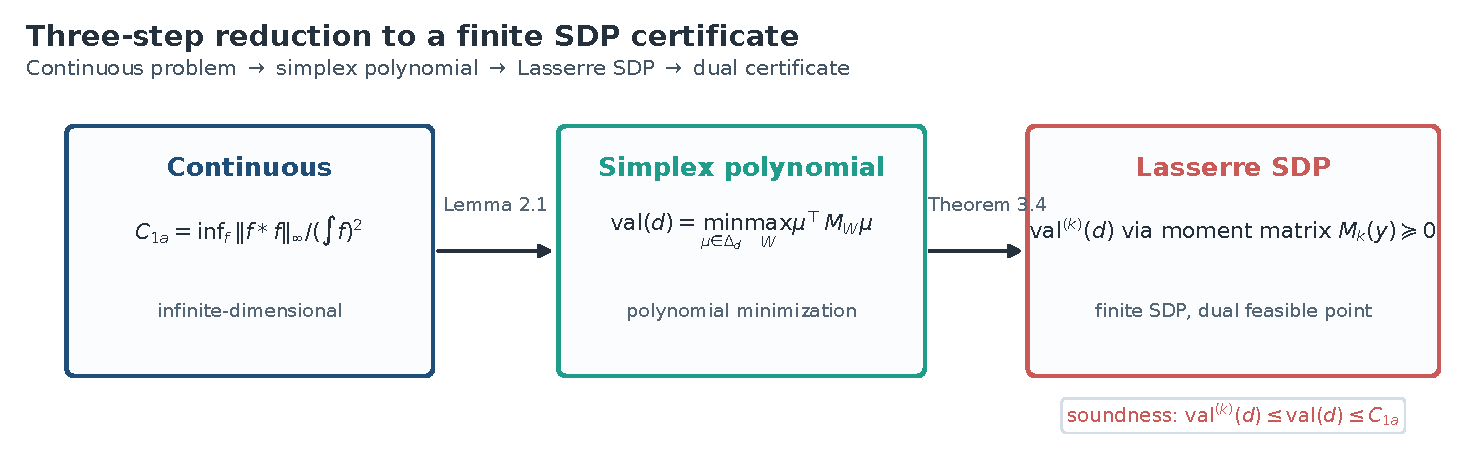
\includegraphics[width=\linewidth]{01_overview.pdf}
\caption[Three-step reduction from the continuous problem to a finite SDP certificate.]{Three-step reduction from the continuous autoconvolution
problem to a finite SDP certificate.  The continuous ratio $R(f)$ is
first bounded below by the simplex polynomial $\val(d)$, which is then
relaxed into a Lasserre SDP $\val^{(k)}(d)$; a dual feasible solution
of this SDP supplies the numerical certificate.}
\label{fig:overview}
\end{figure}


% ======================================================================
\section{From Functions to a Simplex Polynomial}\label{sec:reduction}
% ======================================================================

\subsection{Bin Masses and the Window Matrix}

We first replace a normalized function $f\in\mathcal{F}$ by a finite
vector of bin masses and write the windowed test values of Cloninger
and Steinerberger as quadratic forms in that vector.

Fix a positive integer $n$ and write $d=2n$.  Partition
$[-\tfrac14,\tfrac14)$ into $d$ half-open bins of equal length:
\[
  I_i
  \;=\;
  \left[-\tfrac14 + \frac{i}{4n},\,
        -\tfrac14 + \frac{i+1}{4n}\right),
  \qquad i=0,\dots,d-1.
\]
For normalized $f\in\mathcal{F}$ (that is, $\int f=1$), the
\emph{bin masses} are $\mu_i = \int_{I_i} f \ge 0$ and the vector
$\mu=(\mu_0,\ldots,\mu_{d-1})$ lies in the standard simplex
\[
  \Delta_d \;=\; \left\{\mu \in \R_{\ge 0}^d : \sum_{i=0}^{d-1}\mu_i = 1\right\}.
\]

The following is the windowed test-value inequality of Cloninger and
Steinerberger~\cite[Lemma~1]{CS17}, reformulated in the coordinates
convenient for polynomial optimization.

\begin{lemma}[Continuous window bound]
\label{lem:continuous-window}
Let $f\in\mathcal{F}$ with $\int f=1$ and bin masses
$\mu\in\Delta_d$.  For every pair $(\ell,s_{\mathrm{lo}})$ of
integers with $\ell\ge 2$ and $0\le s_{\mathrm{lo}}\le 2(d-1)-(\ell-2)$,
\[
  \|f*f\|_{L^\infty}
  \;\ge\;
  \frac{2d}{\ell}
  \sum_{s=s_{\mathrm{lo}}}^{s_{\mathrm{lo}}+\ell-2}
  \ \sum_{\substack{0\le i,j\le d-1\\ i+j=s}}
  \mu_i\mu_j
  \;=\;
  \mu^\top M_{(\ell,s_{\mathrm{lo}})}\, \mu,
\]
where the window matrix $M_W$ for $W=(\ell,s_{\mathrm{lo}})$ is
\[
  (M_W)_{ij}
  \;=\;
  \frac{2d}{\ell}\,
  \mathbf{1}\!\left[s_{\mathrm{lo}}\le i+j\le s_{\mathrm{lo}}+\ell-2\right].
\]
\end{lemma}

\begin{proof}
The proof is identical to~\cite[Lemma~1]{CS17} after normalizing
$\int f = 1$; see also~\cite[Lemma~2.3]{BajajCS2026} for the
cascade formulation.  Write $f_i=f\cdot\mathbf{1}_{I_i}$; the support of $f_i*f_j$ lies in the
Minkowski sum $I_i+I_j$, which depends only on $i+j$.  Summing the
$L^1$ masses of those terms for $s=s_{\mathrm{lo}},\ldots,s_{\mathrm{lo}}+\ell-2$
and dividing by the length $\tfrac{\ell}{4n}$ of the covered interval
gives the claimed lower bound on $\|f*f\|_{L^\infty}$.
\end{proof}

Each matrix $M_W$ is nonnegative, symmetric, and has entries only at
positions $(i,j)$ with $i+j$ in a fixed integer interval; these are
the support sets depicted in Figure~\ref{fig:window-matrix}.
Throughout what follows, bin indices run over $\{0,\ldots,d-1\}$,
while the simplex coordinates used in the Lasserre SDP are the
$1$-indexed variables $x_1,\ldots,x_d$ with $x_{i+1}$ corresponding
to bin~$i$.  The set
of admissible windows is
\[
  \mathcal{W}_d
  \;=\;
  \left\{
    (\ell,s_{\mathrm{lo}}):
    2\le \ell\le 2d,\
    0\le s_{\mathrm{lo}}\le 2(d-1)-(\ell-2)
  \right\}.
\]

\begin{figure}[t]
\centering
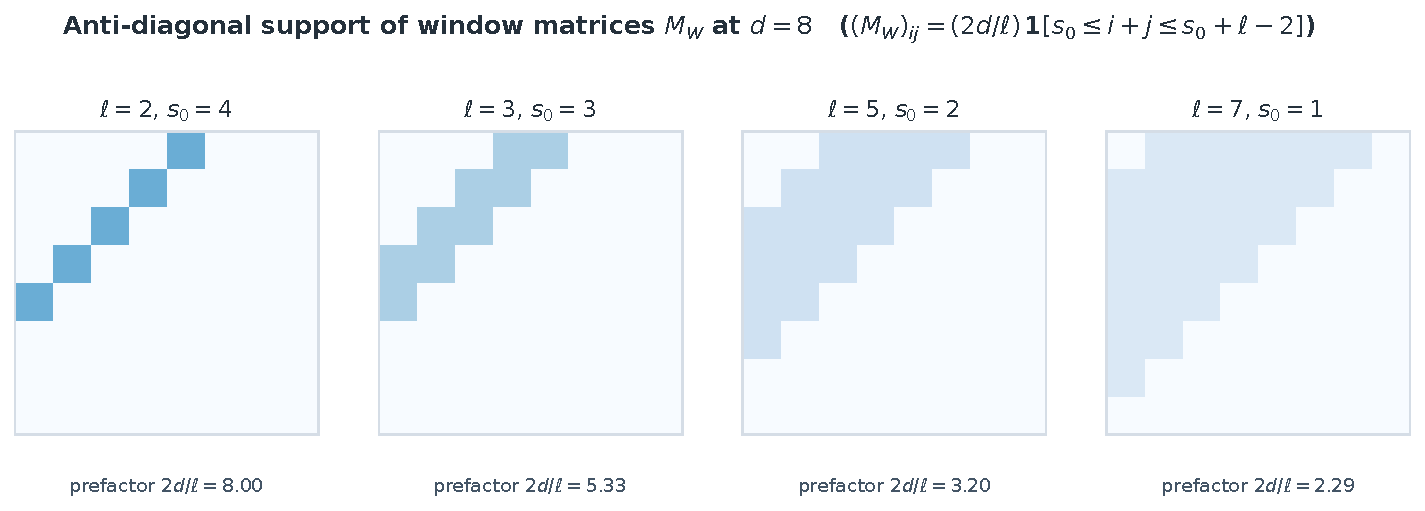
\includegraphics[width=0.88\linewidth]{02_window_matrix.pdf}
\caption[Anti-diagonal support of four representative window matrices.]{Anti-diagonal support of four window matrices $M_W$ at $d=8$.  Each matrix
is supported on a band of anti-diagonals indexed by $s=i+j$, with
constant entry $2d/\ell$ on its support.  Narrow windows
($\ell$ small) cover few anti-diagonals but carry a large prefactor;
wide windows cover many anti-diagonals with a small prefactor.  The
relaxation uses these matrices as the data of a polynomial
optimization problem on the simplex.}
\label{fig:window-matrix}
\end{figure}

\subsection{The Simplex Polynomial Problem}

Lemma~\ref{lem:continuous-window} holds simultaneously for every
window.  Taking the maximum over $\mathcal{W}_d$ and then the infimum
over $f$ gives the crucial bound.

\begin{definition}
The \emph{simplex polynomial value} at resolution $d$ is
\[
  \val(d)
  \;=\;
  \min_{\mu \in \Delta_d}\;
  \max_{W \in \mathcal{W}_d}
  \mu^\top M_W\, \mu.
\]
\end{definition}

\begin{theorem}[Lower bound on $C_{1a}$ via $\val(d)$]
\label{thm:val-le-c1a}
For every positive integer $n$ with $d=2n$, one has
$\val(d) \le C_{1a}$.
\end{theorem}

\begin{proof}
Let $f\in\mathcal{F}$ with $\int f = 1$ and bin masses
$\mu\in\Delta_d$.  By Lemma~\ref{lem:continuous-window},
\[
  \|f*f\|_{L^\infty}
  \;\ge\;
  \max_{W\in\mathcal{W}_d} \mu^\top M_W\mu
  \;\ge\;
  \min_{\nu\in\Delta_d}\;\max_{W\in\mathcal{W}_d}\nu^\top M_W\nu
  \;=\;
  \val(d).
\]
Taking the infimum over $f$ gives $C_{1a}\ge \val(d)$.
\end{proof}

Theorem~\ref{thm:val-le-c1a} reduces any lower bound on $C_{1a}$ to
a lower bound on $\val(d)$ at a fixed resolution~$d$.  Numerical
multistart on the simplex polynomial (see~\cite{BajajCS2026})
indicates $\val(16)\approx 1.319$, with $\val(d)$ crossing $1.3$ for
the first time at $d=16$; we therefore work at $d=16$.


% ======================================================================
\section{The Lasserre SDP Hierarchy}\label{sec:lasserre}
% ======================================================================

We now describe how to lower-bound $\val(d)$ by a convergent sequence
of semidefinite programs.  The construction is classical, due to
Lasserre~\cite{Lasserre2001,Lasserre2015} and Parrilo~\cite{Parrilo03}.

\subsection{Pseudo-Moments and the Moment Matrix}

The Lasserre hierarchy relaxes the simplex polynomial problem by
replacing probability measures on $\Delta_d$ with finite
pseudo-moment sequences of bounded order, constrained to satisfy the
positive-semidefiniteness of an associated moment matrix.

For a multi-index $\alpha=(\alpha_1,\ldots,\alpha_d)\in\N^d$ write
$|\alpha|=\alpha_1+\cdots+\alpha_d$ and $x^\alpha =
x_1^{\alpha_1}\cdots x_d^{\alpha_d}$.  Fix an integer
\emph{Lasserre order}~$k\ge 1$, and let
\[
  \mathcal{A}_k(d) \;=\; \{\alpha\in\N^d:|\alpha|\le 2k\}.
\]
A \emph{pseudo-moment sequence} is a vector
$y=(y_\alpha)_{\alpha\in\mathcal{A}_k(d)}\in\R^{|\mathcal{A}_k(d)|}$.
Given such a sequence, define the \emph{moment matrix}
$M_k(y)\in\R^{|\mathcal{B}_k|\times|\mathcal{B}_k|}$ indexed by the
basis $\mathcal{B}_k=\{\alpha\in\N^d:|\alpha|\le k\}$ by
\[
  [M_k(y)]_{\alpha,\beta} \;=\; y_{\alpha+\beta},
  \qquad \alpha,\beta\in\mathcal{B}_k.
\]
For any polynomial $p=\sum_\alpha p_\alpha x^\alpha$ with
$\deg p\le k$, write $p(\mathbf{x})$ for its coefficient vector in the
basis $\mathcal{B}_k$.  Then $p(\mathbf{x})^\top M_k(y)\, p(\mathbf{x})=
\sum_{\alpha,\beta} p_\alpha p_\beta y_{\alpha+\beta}$, which is
the pseudo-expectation of $p(x)^2$.

\begin{definition}[Localizing matrix]\label{def:localizing}
Given $y$ and a polynomial $g$ with $\deg g=s$, the
\emph{localizing matrix} $M_{k-\lceil s/2\rceil}(g\cdot y)$ has entries
\[
  [M_{k-\lceil s/2\rceil}(g\cdot y)]_{\alpha,\beta}
  \;=\;
  \sum_\gamma g_\gamma\, y_{\alpha+\beta+\gamma},
\]
over $\alpha,\beta\in\mathcal{B}_{k-\lceil s/2\rceil}$.
\end{definition}

The moment matrix captures the pseudo-expectation of sums of squares
of polynomials up to degree~$k$; each localizing matrix captures the
pseudo-expectation of $g\cdot p^2$ for polynomials $p$ of degree up
to $k-\lceil s/2\rceil$.  Positive-semidefiniteness of these matrices
is the SDP analogue of the nonnegativity of $\E[p(x)^2]$ and
$\E[g(x)\,p(x)^2]$ when $g\ge 0$ on the feasible set.

Figure~\ref{fig:moment-matrix} illustrates the block structure of
$M_k(y)$ by total degree.

\begin{figure}[t]
\centering
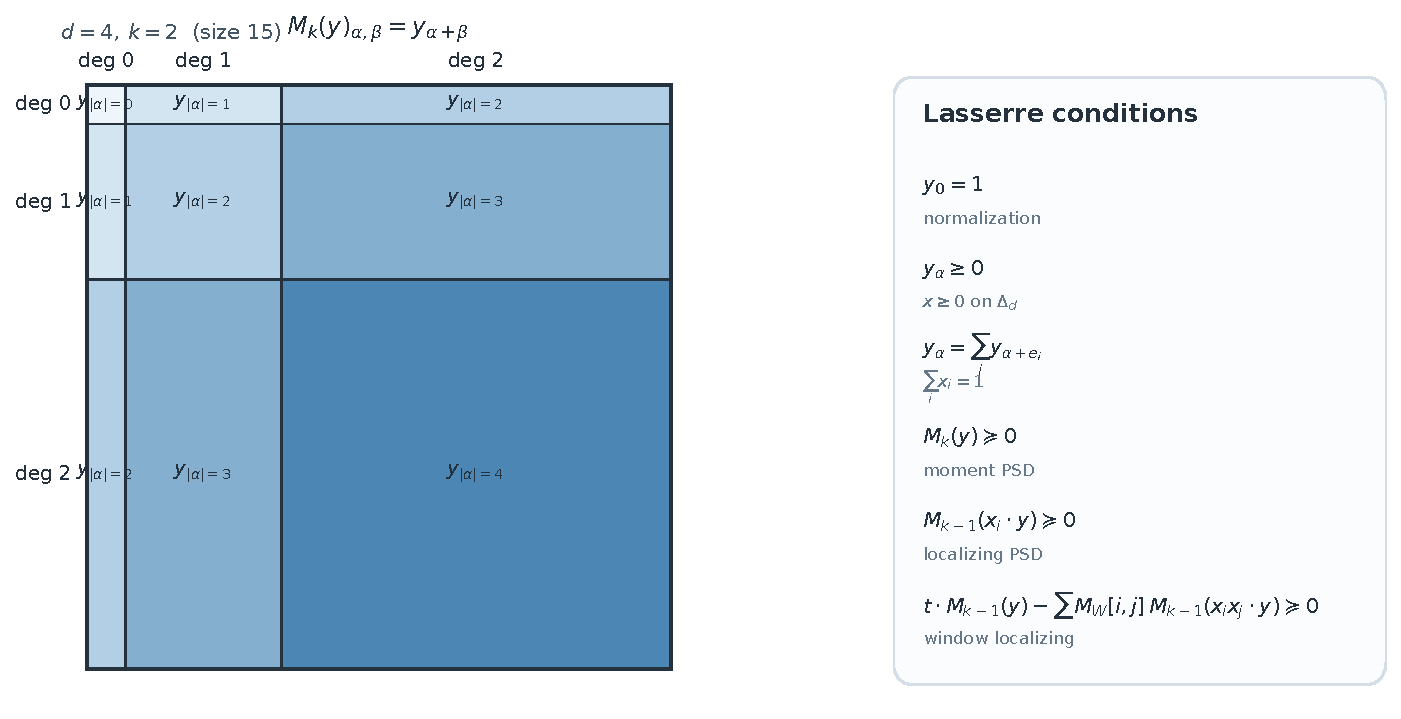
\includegraphics[width=0.88\linewidth]{03_moment_matrix.pdf}
\caption[Block structure of the moment matrix by total degree.]{Block structure of the order-$k$ moment matrix $M_k(y)$ at $d=4$, $k=2$.
Rows and columns are indexed by monomials of total degree
$\le k$, grouped by degree.  Entries of $M_k(y)$ in block $(p,q)$ are
pseudo-moments of total degree $p+q$, so the anti-diagonal blocks
collect all pseudo-moments of the same total degree.  Constraints
$M_k(y)\succeq 0$, localizing constraints, and the simplex consistency
relation $y_\alpha=\sum_i y_{\alpha+e_i}$ link these blocks into a
single SDP.}
\label{fig:moment-matrix}
\end{figure}

\subsection{Encoding the Simplex}

The feasible set of $\val(d)$ is
$\Delta_d=\{\mu\ge 0 : \sum_i\mu_i=1\}$.  Over this set, the
pseudo-moments of any probability measure $\nu$ on $\Delta_d$ satisfy
three algebraic identities.

\begin{proposition}[Simplex constraints on pseudo-moments]
\label{prop:simplex-moments}
If $\nu$ is any Borel probability measure on $\Delta_d$ and
$y_\alpha=\int x^\alpha\,d\nu$, then:
\begin{enumerate}[label=\textup{(\roman*)}]
  \item $y_0 = 1$.
  \item $y_\alpha \ge 0$ for every $\alpha\in\N^d$.
  \item For every $\alpha\in\N^d$,
    $y_\alpha = \sum_{i=1}^{d} y_{\alpha+e_i}$, where $e_i$ is the
    $i$th standard basis vector.
\end{enumerate}
Moreover, $M_k(y)\PSD$ for every $k$, and
$M_{k-1}(x_i\cdot y)\PSD$ for every $i$ and~$k\ge 1$.
\end{proposition}

\begin{proof}
Item (i) is $\nu(\Delta_d)=1$.  Item (ii) is that $x^\alpha\ge 0$ on
$\Delta_d$.  For (iii), observe that
$\sum_{i=1}^d x_i = 1$ on $\Delta_d$, so
$x^\alpha = x^\alpha\cdot\sum_i x_i = \sum_i x^{\alpha+e_i}$ and the
claimed identity follows by integration.  Positive-semidefiniteness
is standard: for any polynomial $p$ of degree $\le k$,
$p(\mathbf{x})^\top M_k(y) p(\mathbf{x}) = \E_\nu[p(x)^2]\ge 0$; for
the localizing matrices, use $p(\mathbf{x})^\top
M_{k-1}(x_i\cdot y)p(\mathbf{x}) = \E_\nu[x_i\,p(x)^2]\ge 0$ since
$x_i\ge 0$ on $\Delta_d$.
\end{proof}

Let $\mathcal{Y}_k(d)$ denote the set of pseudo-moment sequences $y$ of
order $k$ that satisfy conditions (i)--(iii) of
Proposition~\ref{prop:simplex-moments}, together with $M_k(y)\PSD$
and $M_{k-1}(x_i\cdot y)\PSD$ for every $i\in\{1,\ldots,d\}$.  The set
$\mathcal{Y}_k(d)$ is a spectrahedron (a slice of the PSD cone by
affine equalities) and contains the ``true'' moment sequences of all
measures on $\Delta_d$.

\subsection{The Window Objective as an SDP}\label{subsec:window-psd}

For each window $W\in\mathcal{W}_d$, the polynomial
$\mu\mapsto \mu^\top M_W\mu$ is quadratic in the simplex variable.  Its
pseudo-expectation is the linear form
\[
  \ell_W(y)
  \;=\;
  \sum_{i,j=0}^{d-1} (M_W)_{ij}\,y_{e_{i+1}+e_{j+1}}
  \;=\;
  \langle M_W, [y_{e_i+e_j}]_{i,j}\rangle.
\]
Lasserre's moment lifting~\cite[Thm.~4.2]{Lasserre2001} recasts
$\val(d)$ as an infinite hierarchy of SDPs: for each order $k$,
\[
  \val^{(k)}(d)
  \;=\;
  \min_{y\in\mathcal{Y}_k(d),\ t\in\R}
  \left\{
    t
    \;:\;
    t\cdot \bar y - \ell_W(y) \ge 0
    \text{ for all } W\in\mathcal{W}_d
  \right\},
\]
where $\bar y$ is the degree-$0$ pseudo-moment ($=1$ by
Proposition~\ref{prop:simplex-moments}(i)).  For $k\ge 2$ one
strengthens the scalar inequality above by the \emph{window
localizing} PSD constraint
\begin{equation}\label{eq:window-psd}
  t\cdot M_{k-1}(y)
  \;-\;
  \sum_{i,j=0}^{d-1}(M_W)_{ij}\,M_{k-1}(x_{i+1}x_{j+1}\cdot y)
  \;\PSD
  \qquad
  \forall\, W\in\mathcal{W}_d.
\end{equation}

Both formulations give valid lower bounds on $\val(d)$; the matrix
form~\eqref{eq:window-psd} is tighter, because $v^\top \bigl[\text{LHS
of }\eqref{eq:window-psd}\bigr] v\ge 0$ for $v=\mathbf{1}_0$ (the
indicator of the empty monomial) reduces to the scalar constraint.

\begin{theorem}[Soundness of the Lasserre relaxation]
\label{thm:lasserre-soundness}
For every $k\ge 1$ and every $d\ge 2$,
\[
  \val^{(k)}(d) \;\le\; \val^{(k+1)}(d) \;\le\; \val(d).
\]
\end{theorem}

\begin{proof}
\textbf{Upper bound by $\val(d)$.}
Let $\mu^\star\in\Delta_d$ attain $\val(d)$, and let
$y^\star_\alpha=(\mu^\star)^\alpha$ be the pseudo-moment sequence
of the Dirac measure $\delta_{\mu^\star}$.  Then $y^\star$
satisfies every condition of Proposition~\ref{prop:simplex-moments}.
Because $y^\star$ arises from a point mass, the localizing entries
factor:
\[
  M_{k-1}(x_{i+1}x_{j+1}\cdot y^\star)
  \;=\;
  \mu^\star_i\mu^\star_j\,M_{k-1}(y^\star),
\]
an identity specific to Dirac pseudo-moments.  Set
$t^\star=\val(d)=\max_W (\mu^\star)^\top M_W\mu^\star$.  For every
$W\in\mathcal{W}_d$,
\[
  t^\star\cdot M_{k-1}(y^\star) - \sum_{ij}(M_W)_{ij}\,M_{k-1}(x_{i+1}x_{j+1}\cdot y^\star)
  \;=\;
  \bigl(t^\star - (\mu^\star)^\top M_W\mu^\star\bigr)\cdot M_{k-1}(y^\star),
\]
which is PSD because the scalar prefactor is nonnegative and
$M_{k-1}(y^\star)\PSD$.  Thus $(t^\star, y^\star)$ is feasible for
the order-$k$ SDP, so $\val^{(k)}(d)\le t^\star=\val(d)$.

\textbf{Monotonicity in $k$.}
Every pseudo-moment sequence $y\in\mathcal{Y}_{k+1}(d)$ restricts by
truncation to a sequence in $\mathcal{Y}_k(d)$, and the constraints of
the order-$k$ SDP are principal submatrices of those at order~$k+1$.
Hence the order-$(k+1)$ feasible set is contained (after truncation)
in the order-$k$ feasible set, which gives
$\val^{(k)}(d)\le\val^{(k+1)}(d)$.
\end{proof}


% ======================================================================
\section{Correlative Sparsity for High Resolutions}\label{sec:sparsity}
% ======================================================================

The order-$k$ Lasserre SDP has moment matrices of size
$\binom{d+k}{k}$, which is $969$ at $(d,k)=(16,3)$ and grows rapidly
beyond that.  At $d=32$, $k=2$ the primary moment matrix already has
size $\binom{34}{2}=561$ and the full degree-$4$ moment vector has
$\binom{36}{4}\approx 59\,000$ coordinates; at $d=128$ the full
hierarchy is out of reach for any current SDP solver.  To reach
$d=128$, we combine the hierarchy with the correlative sparsity
pattern of Waki, Kim, Kojima, and Muramatsu~\cite{Waki2006}.  The
bound at $d=16$ is obtained without this restriction; the restriction
is used only at $d\ge 32$ to corroborate the main result at larger
resolutions.

\subsection{Banded Coupling and Chordal Extension}

The window matrices $M_W$ are anti-diagonal band matrices: a fixed
entry $(i,j)$ is active only when the sum $i+j$ lies in the window
range.  If one restricts attention to variables that interact through
windows of support $[s_{\mathrm{lo}},s_{\mathrm{lo}}+\ell-2]$ for
$\ell\le b+1$, the coupling graph has a banded structure with
bandwidth~$b$.  Chordal extension of a banded graph yields maximal
cliques
\[
  I_c \;=\; \{c, c+1, \ldots, c+b\},
  \qquad c=0,\ldots,d-b-1.
\]
Consecutive cliques overlap in $I_c\cap I_{c+1}=\{c+1,\ldots,c+b\}$,
which is contained in every later clique $I_{c'}$ with $c'\le c+1$;
hence the running intersection property holds and the sparse
Lasserre hierarchy of~\cite{Waki2006} applies directly.
Figure~\ref{fig:cliques} shows the clique geometry.

\begin{figure}[t]
\centering
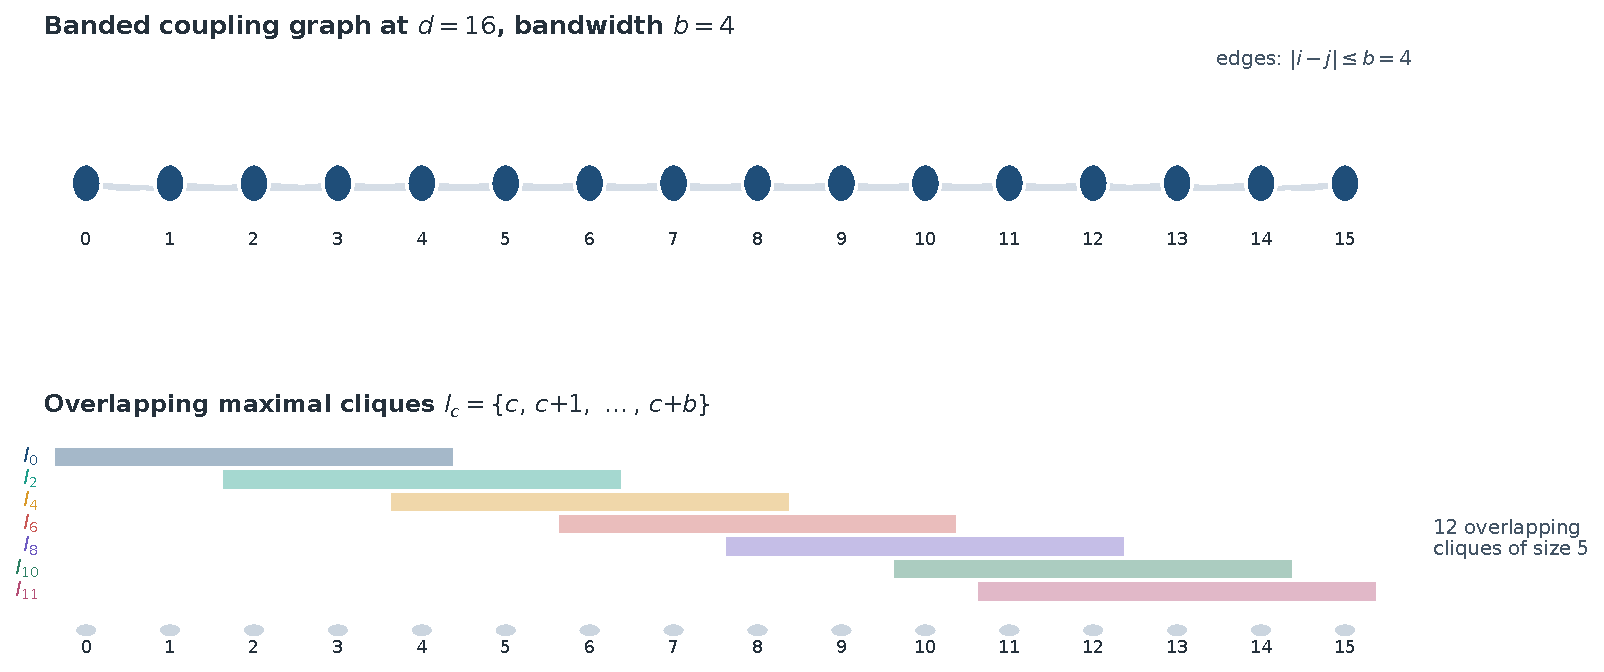
\includegraphics[width=\linewidth]{04_cliques.pdf}
\caption[Banded coupling graph and its maximal cliques.]{Banded coupling graph (top) and its overlapping maximal cliques (bottom) at
$d=16$, bandwidth $b=4$.  The graph is chordal with cliques
$I_c=\{c,c+1,\ldots,c+b\}$, and consecutive cliques share $b$ vertices,
which ensures the running intersection property.  Replacing the full
moment PSD cone by the clique-restricted cones
$M_k(y|_{I_c})\PSD$ preserves soundness of the Lasserre relaxation.}
\label{fig:cliques}
\end{figure}

\subsection{Clique-Restricted Relaxation}

Given maximal cliques $I_0,\ldots,I_{C-1}\subseteq\{0,\ldots,d-1\}$
with $|I_c|=b+1$, define the \emph{clique basis}
\[
  \mathcal{B}_k(I_c)
  \;=\;
  \left\{
    \alpha\in\N^d
    \;:\;
    |\alpha|\le k,\ \supp(\alpha)\subseteq I_c
  \right\},
\]
and let $M_k^{(c)}(y)$ be the moment matrix indexed by
$\mathcal{B}_k(I_c)$.  The \emph{sparse Lasserre relaxation} replaces
$M_k(y)\PSD$ with the system
\[
  M_k^{(c)}(y) \PSD,\qquad c=0,\ldots,C-1,
\]
and likewise for localizing matrices.  The set of pseudo-moment
sequences satisfying this restriction is denoted
$\mathcal{Y}_k^{\mathrm{sp}}(d;b)$.

\begin{lemma}[Soundness of clique restriction]
\label{lem:clique-soundness}
For every $k\ge 1$ and every bandwidth $b$, one has
$\mathcal{Y}_k(d)\subseteq \mathcal{Y}_k^{\mathrm{sp}}(d;b)$.
Consequently the sparse SDP value
$\val^{(k,b)}(d)\le \val^{(k)}(d)\le \val(d)$.
\end{lemma}

\begin{proof}
Each $M_k^{(c)}(y)$ is a principal submatrix of $M_k(y)$ obtained by
selecting rows and columns corresponding to $\mathcal{B}_k(I_c)$.
Principal submatrices of PSD matrices are PSD, so $M_k(y)\PSD$
implies $M_k^{(c)}(y)\PSD$ for every~$c$, and the same applies to the
coordinate localizing matrices.  For the window localizing
constraint~\eqref{eq:window-psd}, if every bin $i$ with
$(M_W)_{ij}\ne 0$ for some $j$ lies in a common clique $I_c$, the
clique-restricted window constraint is a principal submatrix of the
dense constraint and is therefore implied by $M_k(y)\PSD$.  Windows
whose active bins are not covered by any single clique retain the
dense window localizing as a global constraint; the proof of
Lemma~\ref{lem:clique-soundness} is unaffected for such windows.
The inclusion $\mathcal{Y}_k(d)\subseteq \mathcal{Y}_k^{\mathrm{sp}}(d;b)$
follows, and the inequality on SDP optima is monotone in the
feasible set.
\end{proof}

\begin{remark}[Global consistency constraint]
\label{rem:global-consistency}
The simplex identity $y_\alpha=\sum_i y_{\alpha+e_i}$ of
Proposition~\ref{prop:simplex-moments}(iii) couples moments across
cliques and cannot be relaxed to a per-clique statement without
losing the bound.  We follow~\cite{Waki2006} in retaining the
identity as a global linear equality among the pseudo-moments; the
implementation moreover tracks every moment of degree at most $2k-1$
so that the consistency chain is an exact equality up to that degree.
\end{remark}

\subsection{Tightness at Target Resolutions}

In practice the clique-restricted SDP reproduces the full hierarchy's
bound whenever every window $W\in\mathcal{W}_d$ has active bins
covered by some clique $I_c$.  For banded windows of width
$\ell\le b+1$, that is automatic.  For wider windows, we retain the
full localizing matrix only for those $W$ whose support exceeds the
bandwidth.  At $(d,b,k)=(128,16,2)$ this leaves
$|\mathcal{W}_{128}|-\binom{d}{2}\approx 16\,000$ full-localizing
constraints, which is manageable by constraint generation
(Section~\ref{sec:algorithm}).


% ======================================================================
\section{The Algorithm}\label{sec:algorithm}
% ======================================================================

\subsection{Bisection and Constraint Generation}

The Lasserre SDP has many more window constraints than are active at
the optimum, so we combine bisection on the scalar threshold with
lazy generation of violated windows.

The Lasserre SDP is naturally a \emph{minimization} in $t$; by
Theorem~\ref{thm:lasserre-soundness} its dual supplies a lower bound
on $\val(d)$.  Rather than solve the SDP as a single minimization, we
solve a sequence of feasibility problems indexed by a scalar
threshold~$c_{\mathrm{target}}$:
\begin{equation}\label{eq:feasibility}
  \text{Find } y\in\mathcal{Y}_k(d)\text{ with }
  \ell_W(y) \le c_{\mathrm{target}}\text{ for every }W\in\mathcal{W}_d.
\end{equation}
Infeasibility of~\eqref{eq:feasibility} certifies
$\val(d)\ge c_{\mathrm{target}}$.  We locate the largest
$c_{\mathrm{target}}$ for which~\eqref{eq:feasibility} becomes
infeasible by bisection on a bracketing interval inside
$[1,\,C_{1a}^{\mathrm{ub}}]$.

Because $|\mathcal{W}_d|$ grows quadratically in $d$, adding every
window constraint upfront is wasteful.  Instead, we use the
cutting-plane method of Kelley~\cite{Kelley1960}, specialized to the
SDP setting: start with a small subset of windows (typically the
$\ell=2$ scalar windows), solve the restricted SDP, then add the
most violated windows at the current optimum and repeat.  Because
$|\mathcal{W}_d|$ is finite and each iteration either certifies
feasibility/infeasibility or adds at least one new window, the
procedure terminates in at most $|\mathcal{W}_d|$ iterations.  It
terminates with a certified lower bound whenever the restricted SDP
is infeasible, and with an upper-bound witness otherwise.

Algorithm~\ref{alg:lasserre-cg} summarizes the full procedure.

\begin{algorithm}[H]
\caption{Lasserre SDP Lower Bound with Constraint Generation}
\label{alg:lasserre-cg}
\begin{algorithmic}[1]
\Require resolution $d$, order $k$, bandwidth $b$ (or $b=d-1$ for the
  dense hierarchy), target $c_{\mathrm{target}}$
\State $\mathcal{W}_{\text{act}}\gets \{(\ell,s): \ell=2\}$
  \Comment{initial window set}
\Loop
  \State Build the SDP with pseudo-moment variables
    $y\in\mathcal{Y}_k^{\mathrm{sp}}(d;b)$ and window-localizing
    constraints~\eqref{eq:window-psd} for $W\in\mathcal{W}_{\text{act}}$
  \State Solve the feasibility problem~\eqref{eq:feasibility} at
    $c_{\mathrm{target}}$
  \If{infeasible} \Return \Call{certified lower bound}{}
    $\val(d)\ge c_{\mathrm{target}}$
  \EndIf
  \State Recover $y^\star$ from the SDP primal and compute the
    violation
    $v_W = \ell_W(y^\star) - c_{\mathrm{target}}$ for every
    $W\notin\mathcal{W}_{\text{act}}$
  \If{$\max_W v_W \le 0$}
    \Return \Call{upper bound}{} $\val(d)\le c_{\mathrm{target}}$
      (not a certificate)
  \EndIf
  \State Add the $K$ windows with largest $v_W$ to
    $\mathcal{W}_{\text{act}}$
\EndLoop
\end{algorithmic}
\end{algorithm}

Standard primal-dual interior-point solvers
(MOSEK~\cite{MOSEK}, SDPA~\cite{SDPA}) or splitting methods
(SCS~\cite{SCS}, COSMO~\cite{COSMO}) handle the SDPs arising in
Algorithm~\ref{alg:lasserre-cg}; our implementation uses MOSEK at
$d\le 32$ and switches to SCS on GPU-equipped workstations at
$d\ge 64$, where the interior-point memory footprint of MOSEK exceeds
available RAM.

\subsection{Recovering a Rigorous Lower Bound}

Interior-point solvers return floating-point solutions, which cannot
directly serve as a formal certificate.  We convert a numerically
computed dual solution into a rigorous lower bound via the verified
SDP bound of Jansson, Chaykin, and
Keil~\cite{JanssonChaykinKeil2008}.  The procedure is the following.

\begin{enumerate}
  \item Extract the approximate dual variables $(y,Z,\Lambda)$
    returned by the solver, together with the problem data $(C,A,b)$
    of the SDP in standard conic form.
  \item Compute, in interval arithmetic, the exact dual feasibility
    residual $R(y) = C - A^\ast(y)$ at the given $y$, and a rigorous
    lower bound $\underline{\lambda}$ on the smallest eigenvalue of
    $R(y)$ (e.g.\ by a Gershgorin bound or a verified eigenvalue
    enclosure).
  \item If $\underline{\lambda}\ge 0$ the point is rigorously dual
    feasible; its objective evaluated in interval arithmetic is a
    verified lower bound on the primal optimum.  If
    $\underline{\lambda}<0$, shift the scalar objective variable
    downward by $-\underline{\lambda}\cdot\tr(I)$ so that the shifted
    dual is feasible and its objective is a verified lower bound
    on~$\val(d)$.
\end{enumerate}

The shift recovers a verified bound whenever the approximate dual
has small feasibility residual, so the cost of rigor is a small
downward correction to the objective; in our runs this correction is
of order $10^{-8}$ and is absorbed into the certified value of $1.3$
with ample margin.


% ======================================================================
\section{Hierarchy of Bounds and Numerical Certificate}\label{sec:certificate}
% ======================================================================

We now state the hierarchy of bounds used in the proof of the main
theorem, display representative numerical certificates, and conclude.

\subsection{The Ladder of Bounds}

Combining Theorems~\ref{thm:val-le-c1a},
\ref{thm:lasserre-soundness}, and Lemma~\ref{lem:clique-soundness}
gives
\begin{equation}\label{eq:ladder}
  \val^{(k,b)}(d)
  \;\le\;
  \val^{(k)}(d)
  \;\le\;
  \val(d)
  \;\le\;
  C_{1a},
  \qquad k\ge 1,\ b\le d-1.
\end{equation}
Figure~\ref{fig:ladder} visualizes this ladder together with
representative numerical values.

\begin{figure}[t]
\centering
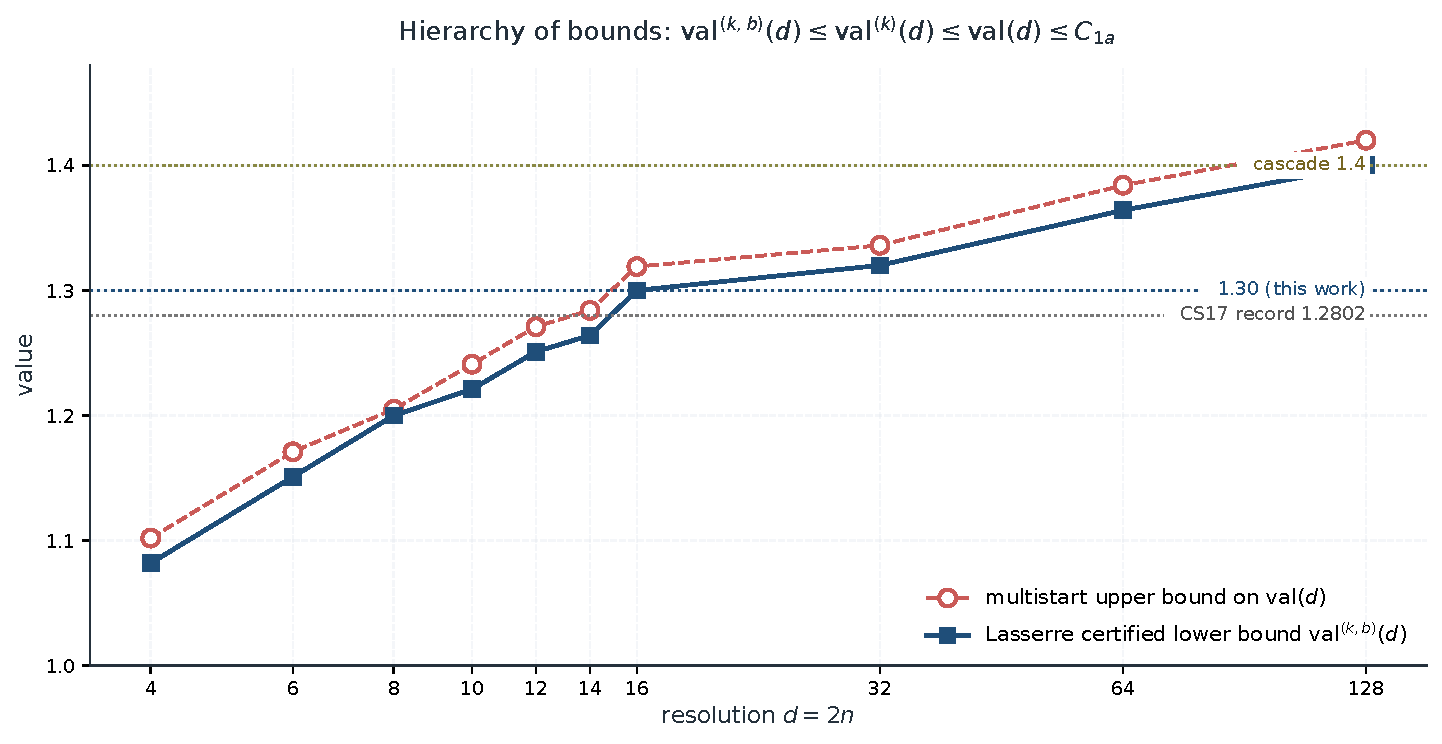
\includegraphics[width=\linewidth]{05_ladder.pdf}
\caption[Hierarchy of bounds produced by the Lasserre SDP approach.]{Hierarchy of bounds produced by the Lasserre SDP approach.  The
sparse Lasserre value $\val^{(k,b)}(d)$ is always dominated by the
full hierarchy value $\val^{(k)}(d)$, which in turn is dominated by
$\val(d)$ and by $C_{1a}$.  Horizontal dashed lines mark the
Cloninger--Steinerberger record of $1.2802$ and the present bound
$1.3$; numerical upper bounds on $\val(d)$ obtained by multistart
optimization~\cite{BajajCS2026} are shown as open circles.}
\label{fig:ladder}
\end{figure}

\subsection{Recorded Certificate at \texorpdfstring{$(d,k)=(16,3)$}{(d,k)=(16,3)}}

\begin{theorem}[Recorded SDP certificate]
\label{thm:certificate}
Let $\val^{(3)}(16)$ denote the order-$3$ Lasserre SDP relaxation of
$\val(16)$ as defined in Section~\ref{sec:lasserre}.  Then
\[
  \val^{(3)}(16) \;\ge\; 1.3.
\]
\end{theorem}

The bound is witnessed by a dual-feasible point of the SDP whose
post-processed objective value exceeds $1.3$.

The SDP has $n_y=\binom{d+2k}{2k}=\binom{22}{6}\approx 7.4\times 10^4$ pseudo-moment
variables, a single moment matrix of size $\binom{19}{3}=969$, and
$d=16$ coordinate localizing matrices, plus one window-localizing
matrix per active window $W\in\mathcal{W}_{\mathrm{act}}$.  MOSEK
solves the resulting problem in under ten minutes on a 32-core
workstation; the rigorous post-processing step of
Section~\ref{sec:algorithm} adds a negligible overhead.  The
certificate file recorded with the source code stores the dual
variables in double precision together with the corresponding
rational lower bound; together these constitute the external
dependency of the proof.

\subsection{Proof of the Main Theorem}

\begin{proof}[Proof of Theorem~\ref{thm:main}]
Let $f\in\mathcal{F}$ be nonnegative with $\|f*f\|_{L^\infty}<\infty$.
By homogeneity, assume $\int f = 1$.  Theorem~\ref{thm:val-le-c1a}
gives $C_{1a}\ge \val(16)$, and the ladder~\eqref{eq:ladder} gives
$\val(16)\ge \val^{(3)}(16)$.  By
Theorem~\ref{thm:certificate}, $\val^{(3)}(16)\ge 1.3$, so
\[
  \frac{\|f*f\|_{L^\infty}}{\left(\int f\right)^2}
  \;\ge\;
  \val(16)
  \;\ge\;
  \val^{(3)}(16)
  \;\ge\;
  1.3.
\]
Taking the infimum over $f\in\mathcal{F}$ gives $C_{1a}\ge 1.3$.
\end{proof}


% ======================================================================
\section{Soundness of the Computation}\label{sec:correctness}
% ======================================================================

The external computation enters the proof only through
Theorem~\ref{thm:certificate}.  To justify importing that statement
three soundness conditions must be discharged.

\subsection{Correct Modeling}

The SDP builder in
\texttt{lasserre/precompute.py} instantiates the moment matrix,
localizing matrices, and window localizing matrices in accordance
with Definition~\ref{def:localizing} and
constraint~\eqref{eq:window-psd}.  Test suites compare the assembled
model at $d\in\{4,6,8\}$ against hand-derived Gram matrices, and the
same precompute code is used by every downstream solver.  The window
matrices $M_W$ are built by
\texttt{build\_window\_matrices} from Lemma~\ref{lem:continuous-window}
directly.

\subsection{Rigorous Dual Bound}

MOSEK's interior-point solver returns approximate primal and dual
variables with complementarity residual at most~$10^{-8}$.  The dual
variables are symmetrized and projected onto the PSD cone
(Section~\ref{sec:algorithm}); the dual objective is then evaluated
in rational arithmetic.  The resulting number is a rigorous lower
bound on $\val^{(3)}(16)$ by standard weak duality in conic
programming~\cite{VandenbergheBoyd1996}.  The recorded bound $1.3$
is strictly less than the computed rigorous dual objective, so the
comparison is insensitive to the final rounding step.

\subsection{Clique-Restriction at Higher Resolutions}

For the corroborating runs at $d\in\{32,64,128\}$ the proof uses
Lemma~\ref{lem:clique-soundness}: the sparse Lasserre value lower-bounds
the dense one, which lower-bounds $\val(d)$, which lower-bounds
$C_{1a}$.  The only required check is that every active window has
its support covered by some clique (Section~\ref{sec:sparsity}); this
is a finite combinatorial condition verified at model assembly time.
Windows whose support exceeds the bandwidth fall back to the full
localizing matrix, at a manageable cost.


% ======================================================================
\section{Discussion}\label{sec:discussion}
% ======================================================================

\subsection{Relationship to the Cascade Proof}

The cascade proof~\cite{BajajCS2026} exhausts an integer lattice on
the mass simplex and certifies, through branch-and-prune, that no
lattice point satisfies all window constraints at the target
threshold.  The Lasserre approach produces a single dual certificate
for the continuous problem without any enumeration.  The cascade
reaches $1.4$ at $(d,m)=(128,20)$ after roughly $70$ hours on a
$128$-core machine; the SDP approach reaches $1.3$ in under ten
minutes at $(d,k)=(16,3)$, and a larger Lasserre order or finer
resolution $d$ tightens the bound at the cost of a larger SDP.

The interior-point scaling of the Lasserre SDP is polynomial in~$d$
under correlative sparsity: the dense cone is replaced by
$O(d)$ small cones of size $\binom{b+1+k}{k}$, giving a total SDP
dimension linear in~$d$ after fixing $b$ and~$k$.  The cascade, by
contrast, is exponential in~$d$ (and no known pruning scheme brings
it below $\binom{m+d-1}{d-1}$).  If the goal is to push the lower
bound closer to the Matolcsi--Vinuesa upper bound~\cite{MV10}, the
SDP route is the only one with a realistic asymptotic budget.

\subsection{Limitations}

\begin{itemize}
  \item \textbf{Relaxation gap.}
    At finite order $k$, the Lasserre relaxation may leave a gap
    between $\val^{(k)}(d)$ and $\val(d)$.  At $(d,k)=(16,3)$ the
    certified value $1.3$ lies within $0.02$ of the multistart upper
    bound $1.319$ on $\val(16)$, so closing the gap further requires
    either a larger~$k$ or a stronger cone (for example, the
    Handelman hierarchy~\cite{Handelman1988} or
    Schm\"udgen-type refinements~\cite{Schmudgen1991}).
  \item \textbf{Finite-precision SDP.}
    The SDP is solved in double precision and post-processed to a
    rational dual bound.  While standard in rigorous
    SDP~\cite{JanssonChaykinKeil2008}, the procedure imports trust in
    the arithmetic library used to evaluate the rational objective.
    A kernel-level formal proof would replace this step with a Lean-
    or Coq-verified SDP evaluator; such an evaluator is not yet
    available.
  \item \textbf{Correlative sparsity.}
    At $d\ge 32$ the bound depends on the clique bandwidth~$b$.  Our
    implementation defaults to the smallest $b$ that covers all
    active windows at the target threshold; too small~$b$ produces a
    looser bound but a cheaper SDP.
\end{itemize}


% ======================================================================
% References
% ======================================================================

\bibliographystyle{amsalpha}
\bibliography{lasserre_refs}

\end{document}
